%
% This document contains the chapter about DC analysis.
%
% Copyright (C) 2003, 2004, 2005 Stefan Jahn <stefan@lkcc.org>
% Copyright (C) 2004 Michael Margraf <Michael.Margraf@alumni.TU-Berlin.DE>
%
% Permission is granted to copy, distribute and/or modify this document
% under the terms of the GNU Free Documentation License, Version 1.1
% or any later version published by the Free Software Foundation.
%

\chapter{DC Analysis}
%\addcontentsline{toc}{chapter}{DC Analysis}

\section{Modified Nodal Analysis}
%\addcontentsline{toc}{section}{Modified Nodal Analysis}
\label{sec:MNA}

Many different kinds of network element are encountered in network
analysis.  For circuit analysis it is necessary to formulate equations
for circuits containing as many different types of network elements as
possible.  There are various methods for equation formulation for a
circuit.  These are based on three types of equations found in circuit
theory:

\begin{itemize}
\item equations based on Kirchhoff's voltage law (KVL)
\item equations based on Kirchhoff's current law (KCL)
\item branch constitutive equations
\end{itemize}

The equations have to be formulated (represented in a computer
program) automatically in a simple, comprehensive manner.  Once
formulated, the system of equations has to be solved.  There are two
main aspects to be considered when choosing algorithms for this
purpose: accuracy and speed.  The MNA, briefly for \textbf{M}odified
\textbf{N}odal \textbf{A}nalysis, has been proved to accomplish these
tasks.

MNA applied to a circuit with passive elements, independent current
and voltage sources and active elements results in a matrix equation
of the form:
\begin{equation}
\left[A\right] \cdot \left[x\right] = \left[z\right]
\end{equation}

For a circuit with N nodes and M independent voltage sources:

\begin{itemize}

\item The A matrix
\begin{itemize}
\item
is (N+M)$\times$(N+M) in size, and consists only of known quantities
\item
the N$\times$N part of the matrix in the upper left:
\begin{itemize}
\item
has only passive elements
\item
elements connected to ground appear only on the diagonal
\item
elements not connected to ground are both on the diagonal and
off-diagonal terms
\end{itemize}
\item
the rest of the A matrix (not included in the N$\times$N upper left
part) contains only 1, -1 and 0 (other values are possible if there
are dependent current and voltage sources)
\end{itemize}

\item The x matrix
\begin{itemize}
\item
is an (N+M)$\times$1 vector that holds the unknown quantities (node
voltages and the currents through the independent voltage sources)
\item
the top N elements are the n node voltages
\item
the bottom M elements represent the currents through the M independent
voltage sources in the circuit
\end{itemize}

\item The z matrix
\begin{itemize}
\item
is an (N+M)$\times$1 vector that holds only known quantities
\item
the top N elements are either zero or the sum and difference of
independent current sources in the circuit
\item
the bottom M elements represent the M independent voltage sources in
the circuit
\end{itemize}
\end{itemize}

The circuit is solved by a simple matrix manipulation:
\begin{equation}
\left[x\right] = \left[A\right]^{-1} \cdot \left[z\right]
\end{equation}

Though this may be difficult by hand, it is straightforward and so is
easily done by computer.

\subsection{Generating the MNA matrices}
%\addcontentsline{toc}{subsection}{Generating the MNA matrices}

The following section is an algorithmic approach to the concept of the
Modified Nodal Analysis.  There are three matrices we need to
generate, the A matrix, the x matrix and the z matrix.  Each of these
will be created by combining several individual sub-matrices.

\subsection{The A matrix}
%\addcontentsline{toc}{subsection}{The A matrix}

The A matrix will be developed as the combination of 4 smaller
matrices, G, B, C, and D.

\begin{equation}
A =
\begin{bmatrix}
G & B\\
C & D
\end{bmatrix}
\end{equation}

The A matrix is (M+N)$\times$(M+N) (N is the number of nodes, and M is the
number of independent voltage sources) and:

\begin{itemize}
\item
the G matrix is N$\times$N and is determined by the interconnections
between the circuit elements
\item
the B matrix is M$\times$N and is determined by the connection of the voltage
sources
\item
the C matrix is N$\times$M and is determined by the connection of
the voltage sources (B and C are closely related, particularly when
only independent sources are considered)
\item
the D matrix is M$\times$M and is zero if only independent sources are
considered
\end{itemize}

\subsubsection{Rules for making the G matrix}
%\addcontentsline{toc}{subsubsection}{Rules for making the G matrix}

The G matrix is an N$\times$N matrix formed in two steps.

\begin{enumerate}
\item
Each element in the diagonal matrix is equal to the sum of the
conductance (one over the resistance) of each element connected to the
corresponding node.  So the first diagonal element is the sum of
conductances connected to node 1, the second diagonal element is the
sum of conductances connected to node 2, and so on.
\item
The off diagonal elements are the negative conductance of the element
connected to the pair of corresponding node.  Therefore a resistor
between nodes 1 and 2 goes into the G matrix at location (1,2) and
locations (2,1).
\end{enumerate}

If an element is grounded, it will only have contribute to one entry
in the G matrix -- at the appropriate location on the diagonal.  If it
is ungrounded it will contribute to four entries in the matrix -- two
diagonal entries (corresponding to the two nodes) and two off-diagonal
entries.

\subsubsection{Rules for making the B matrix}
%\addcontentsline{toc}{subsubsection}{Rules for making the B matrix}

The B matrix is an M$\times$N matrix with only 0, 1 and -1 elements.
Each location in the matrix corresponds to a particular voltage source
(first dimension) or a node (second dimension).  If the positive
terminal of the ith voltage source is connected to node k, then the
element (i,k) in the B matrix is a 1.  If the negative terminal of the
ith voltage source is connected to node k, then the element (i,k) in
the B matrix is a -1.  Otherwise, elements of the B matrix are zero.

\addvspace{12pt}

If a voltage source is ungrounded, it will have two elements in the B
matrix (a 1 and a -1 in the same column).  If it is grounded it will
only have one element in the matrix.

\subsubsection{Rules for making the C matrix}
%\addcontentsline{toc}{subsubsection}{Rules for making the C matrix}

The C matrix is an N$\times$M matrix with only 0, 1 and -1 elements.
Each location in the matrix corresponds to a particular node (first
dimension) or voltage source (second dimension).  If the positive
terminal of the ith voltage source is connected to node k, then the
element (k,i) in the C matrix is a 1.  If the negative terminal of the
ith voltage source is connected to node k, then the element (k,i) in
the C matrix is a -1.  Otherwise, elements of the C matrix are zero.

\addvspace{12pt}

In other words, the C matrix is the transpose of the B matrix.  This
is not the case when dependent sources are present.

\subsubsection{Rules for making the D matrix}
%\addcontentsline{toc}{subsubsection}{Rules for making the D matrix}

The D matrix is an M$\times$M matrix that is composed entirely of
zeros.  It can be non-zero if dependent sources are considered.

\subsection{The x matrix}
\label{sec:xmatrix}
%\addcontentsline{toc}{subsection}{The x matrix}

The x matrix holds our unknown quantities and will be developed as the
combination of 2 smaller matrices v and j.  It is considerably easier
to define than the A matrix.

\begin{equation}
x =
\begin{bmatrix}
v\\
j
\end{bmatrix}
\end{equation}

The x matrix is 1$\times$(M+N) (N is the number of nodes, and M is the
number of independent voltage sources) and:

\begin{itemize}
\item
the v matrix is 1$\times$N and hold the unknown voltages
\item
the j matrix is 1$\times$M and holds the unknown currents through the
voltage sources
\end{itemize}

\subsubsection{Rules for making the v matrix}
%\addcontentsline{toc}{subsubsection}{Rules for making the v matrix}

The v matrix is an 1$\times$N matrix formed of the node voltages.
Each element in v corresponds to the voltage at the equivalent node in
the circuit (there is no entry for ground -- node 0).

\addvspace{12pt}

For a circuit with N nodes we get:

\begin{equation}
v =
\begin{bmatrix}
v_{1}\\
v_{2}\\
\vdots\\
v_{N}\\
\end{bmatrix}
\end{equation}

\subsubsection{Rules for making the j matrix}
%\addcontentsline{toc}{subsubsection}{Rules for making the j matrix}

The j matrix is an 1$\times$M matrix, with one entry for the current
through each voltage source.  So if there are M voltage sources
$V_{1}$, $V_{2}$ through $V_{M}$, the j matrix will be:

\begin{equation}
j =
\begin{bmatrix}
i_{V_{1}}\\
i_{V_{2}}\\
\vdots\\
i_{V_{M}}\\
\end{bmatrix}
\end{equation}

\subsection{The z matrix}
%\addcontentsline{toc}{subsection}{The z matrix}

The z matrix holds our independent voltage and current sources and
will be developed as the combination of 2 smaller matrices i and e.
It is quite easy to formulate.

\begin{equation}
z =
\begin{bmatrix}
i\\
e
\end{bmatrix}
\end{equation}

The z matrix is 1$\times$(M+N) (N is the number of nodes, and M is the
number of independent voltage sources) and:

\begin{itemize}
\item
the i matrix is 1$\times$N and contains the sum of the currents through the
passive elements into the corresponding node (either zero, or the sum
of independent current sources)
\item
the e matrix is 1$\times$M and holds the values of the independent
voltage sources
\end{itemize}

\subsubsection{Rules for making the i matrix}
%\addcontentsline{toc}{subsubsection}{Rules for making the i matrix}

The i matrix is an 1$\times$N matrix with each element of the matrix
corresponding to a particular node.  The value of each element of i is
determined by the sum of current sources into the corresponding node.
If there are no current sources connected to the node, the value is
zero.

\subsubsection{Rules for making the e matrix}
%\addcontentsline{toc}{subsubsection}{Rules for making the e matrix}

The e matrix is an 1$\times$M matrix with each element of the matrix
equal in value to the corresponding independent voltage source.

\subsection{A simple example}
%\addcontentsline{toc}{subsection}{A simple example}

The example given in fig. \ref{fig:MNAexample} illustrates applying
the rules for building the MNA matrices and how this relates to basic
equations used in circuit analysis.

\begin{figure}[ht]
\begin{center}
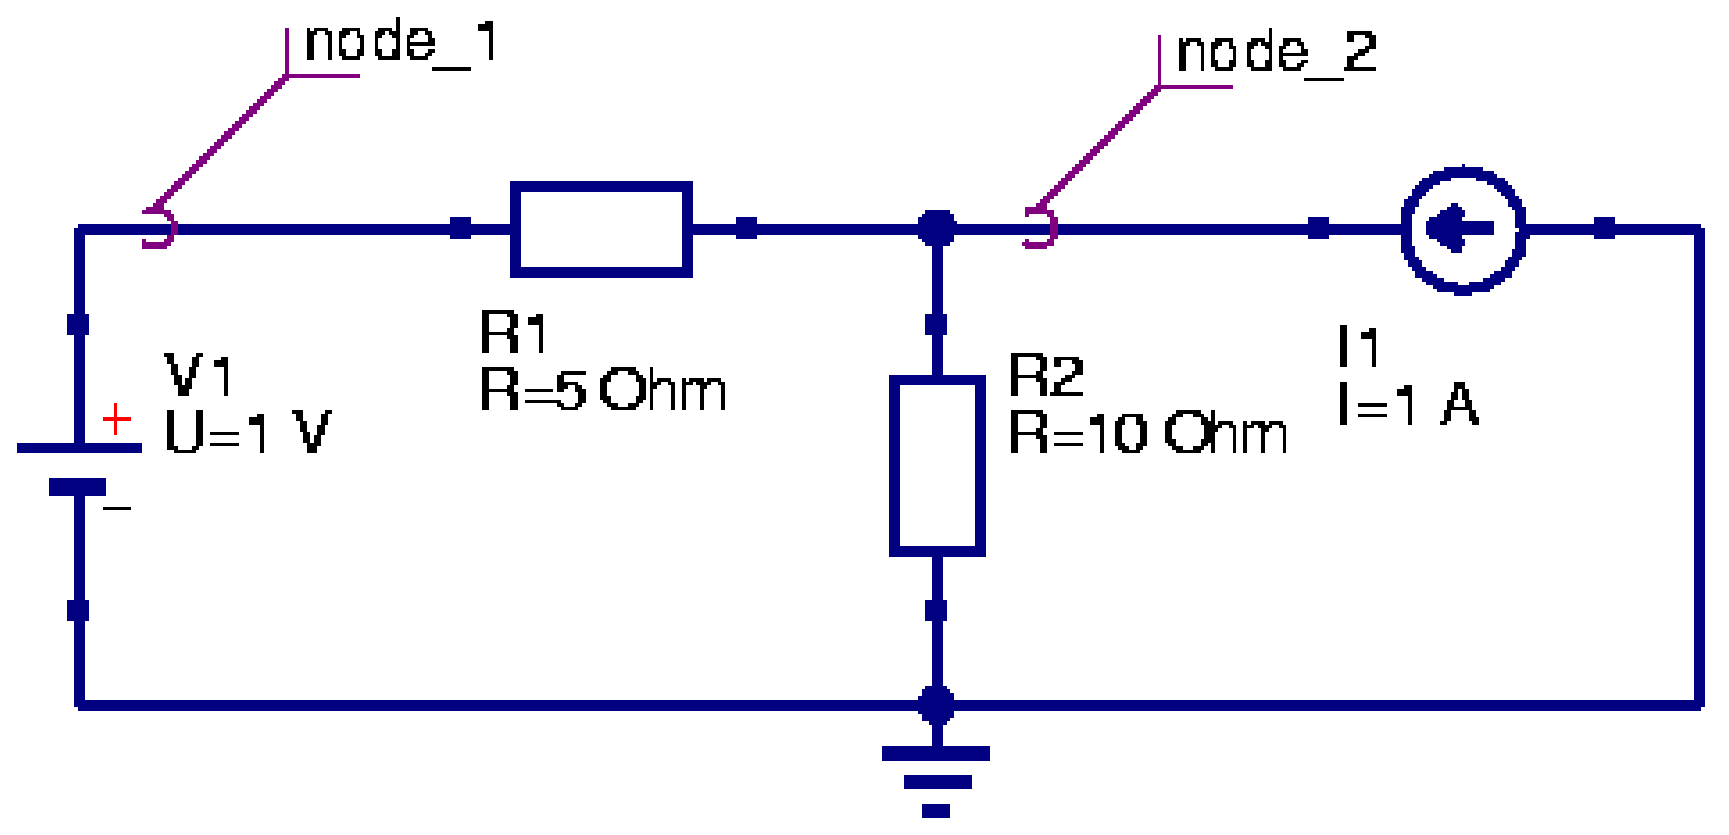
\includegraphics[width=10cm]{MNAexample}
\end{center}
\caption{example circuit applied to modified nodal analysis}
\label{fig:MNAexample}
\end{figure}
\FloatBarrier

\subsubsection{Going through the MNA algorithm}
%\addcontentsline{toc}{subsubsection}{Going through the MNA algorithm}

The G matrix is a 2$\times$2 matrix because there are 2 different
nodes apart from ground which is the reference node.  On the diagonal
you find the sum of the elements conductances connected to the nodes 1
and 2.  The off-diagonal matrix entries contain the negative
conductances of the elements connected between two nodes.

\begin{equation}
G =
\begin{bmatrix}
\frac{1}{R_{1}} & -\frac{1}{R_{1}}\\
-\frac{1}{R_{1}} & \frac{1}{R_{1}} + \frac{1}{R_{2}}
\end{bmatrix}
=
\begin{bmatrix}
0.2 & -0.2\\
-0.2 & 0.3
\end{bmatrix}
\end{equation}

The B matrix (which is transposed to C) is a 1$\times$2 matrix because
there is one voltage source and 2 nodes.  The positive terminal of the
voltage source $V_{1}$ is connected to node 1.  That is why

\begin{equation}
B = C^{T} =
\begin{bmatrix}
1\\
0
\end{bmatrix}
\end{equation}

and the D matrix is filled with zeros only because there are no dependent
(active and controlled) devices in the example circuit.

\begin{equation}
D =
\begin{bmatrix}
0
\end{bmatrix}
\end{equation}

The x matrix is a 1$\times$3 matrix.  The MNA equations deliver a
solution for the unknown voltages at each node in a circuit except the
reference node and the currents through each voltage source.

\begin{equation}
x =
\begin{bmatrix}
v_{1}\\
v_{2}\\
i_{V_{1}}
\end{bmatrix}
\end{equation}

The z matrix is according to the rules for building it a 1$\times$3
matrix.  The upper two entries are the sums of the currents flowing
into node 1 and node 2.  The lower entry is the voltage value of the
voltage source $V_{1}$.

\begin{equation}
z =
\begin{bmatrix}
0\\
I_{1}\\
U_{1}
\end{bmatrix}
=
\begin{bmatrix}
0\\
1\\
1
\end{bmatrix}
\end{equation}

According to the MNA algorithm the equation system is represented by

\begin{equation}
\left[A\right] \cdot \left[x\right] = \left[z\right]
\end{equation}

which is equivalent to

\begin{equation}
\begin{bmatrix}
G & B\\
C & D
\end{bmatrix}
\cdot
\begin{bmatrix}
x
\end{bmatrix}
=
\begin{bmatrix}
z
\end{bmatrix}
\label{eq:MNAexample}
\end{equation}

In the example eq. \eqref{eq:MNAexample} expands to:

\begin{equation}
\begin{bmatrix}
\frac{1}{R_{1}} & -\frac{1}{R_{1}} & 1\\
-\frac{1}{R_{1}} & \frac{1}{R_{1}} + \frac{1}{R_{2}} & 0\\
1 & 0 & 0
\end{bmatrix}
\cdot
\begin{bmatrix}
v_{1}\\
v_{2}\\
i_{V_{1}}
\end{bmatrix}
=
\begin{bmatrix}
0\\
I_{1}\\
U_{1}
\end{bmatrix}
\label{eq:MNAfull}
\end{equation}

The equation systems to be solved is now defined by the following
matrix representation.

\begin{equation}
\begin{bmatrix}
0.2 & -0.2 & 1\\
-0.2 & 0.3 & 0\\
1 & 0 & 0
\end{bmatrix}
\cdot
\begin{bmatrix}
v_{1}\\
v_{2}\\
i_{V_{1}}
\end{bmatrix}
=
\begin{bmatrix}
0\\
1\\
1
\end{bmatrix}
\end{equation}

Using matrix inversion the solution vector x writes as follows:

\begin{equation}
\left[x\right] = 
\left[A\right]^{-1}\cdot \left[z\right] = 
\begin{bmatrix}
v_{1}\\
v_{2}\\
i_{V_{1}}
\end{bmatrix}
=
\begin{bmatrix}
1\\
4\\
0.6
\end{bmatrix}
\label{eq:MNAresult}
\end{equation}

The result in eq. (\ref{eq:MNAresult}) denotes the current through the
voltage source $V_{1}$ is $0.6\ampere$, the voltage at node 1 is
$1\volt$ and the voltage at node 2 is $4\volt$.

\subsubsection{How the algorithm relates to basic equations in circuit analysis}
%\addcontentsline{toc}{subsubsection}{How the algorithm relates to basic equations in circuit analysis}

Expanding the matrix representation in eq. (\ref{eq:MNAfull}) to a set
of equations denotes the following equation system consisting of 3 of
them.

\begin{align}
\rm{I:}& \qquad 0 = \frac{1}{R_{1}}\cdot v_{1} - \frac{1}{R_{1}}\cdot v_{2} + i_{V_{1}}& \text{KCL at node 1}\\
\rm{II:}& \qquad I_{1} = -\frac{1}{R_{1}}\cdot v_{1} + \left(\frac{1}{R_{1}} + \frac{1}{R_{2}}\right)\cdot v_{2}& \text{KCL at node 2}\\
\rm{III:}& \qquad U_{1} = v_{1}& \text{constitutive equation}
\end{align}

Apparently eq. I and eq. II conform to Kirchhoff's current law at the
nodes 1 and 2.  The last equation is just the constitutive equation
for the voltage source $V_{1}$.  There are three unknowns ($v_{1}$,
$v_{2}$ and $i_{V_{1}}$) and three equations, thus the system should
be solvable.

\addvspace{12pt}

Equation III indicates the voltage at node 1 is $1\volt$.  Applying
this result to eq. II and transposing it to $v_{2}$ (the voltage at
node 2) gives

\begin{equation}
v_{2} = \frac{I_{1} + \frac{1}{R_{1}}\cdot U_{1}}{\frac{1}{R_{1}} + \frac{1}{R_{2}}} = 4\volt
\end{equation}

The missing current through the voltage source $V_{1}$ can be computed
using both the results $v_{2} = 4\volt$ and $v_{1} = 1\volt$ by
transforming equation I.

\begin{equation}
i_{V_{1}} = \frac{1}{R_{1}}\cdot v_{2} - \frac{1}{R_{1}}\cdot v_{1} = 0.6\ampere
\end{equation}

The small example, shown in fig. \ref{fig:MNAexample}, and the
excursus into artless math verifies that the MNA algorithm and classic
electrical handiwork tend to produce the same results.

\section{Solving linear equation systems}
%\addcontentsline{toc}{section}{Solving linear equation systems}

When dealing with non-linear networks the number of equation systems
to be solved depends on the required precision of the solution and the
average necessary iterations until the solution is stable.  This
emphasizes the meaning of the solving procedures choice for different
problems.

\addvspace{12pt}

The equation systems
\begin{equation}
\left[A\right] \cdot \left[x\right] = \left[z\right]
\end{equation}
solution can be written as
\begin{equation}
\left[x\right] = \left[A\right]^{-1} \cdot \left[z\right]
\end{equation}

\subsection{Matrix inversion}
%\addcontentsline{toc}{subsection}{Matrix inversion}

The elements $\beta_{\mu\nu}$ of the inverse of the matrix $A$ are
\begin{equation}
\beta_{\mu\nu} = \frac{A_{\mu\nu}}{det A}
\end{equation}
whereas $A_{\mu\nu}$ is the matrix elements $a_{\mu\nu}$ cofactor.
The cofactor is the sub determinant (i.e. the minor) of the element
$a_{\mu\nu}$ multiplied with $(-1)^{\mu + \nu}$.  The determinant of a
square matrix can be recursively computed by either of the following
equations.
\begin{align}
det A = \sum_{\mu = 1}^{n} a_{\mu\nu}\cdot A_{\mu\nu}
\quad &\text{using the $\nu$-th column}\\
det A = \sum_{\nu = 1}^{n} a_{\mu\nu}\cdot A_{\mu\nu}
\quad &\text{using the $\mu$-th row}
\end{align}

This method is called the Laplace expansion.  In order to save
computing time the row or column with the most zeros in it is used for
the expansion expressed in the above equations.  A sub determinant
$(n-1)$-th order of a matrix's element $a_{\mu\nu}$ of $n$-th order is
the determinant which is computed by canceling the $\mu$-th row and
$\nu$-th column.  The following example demonstrates calculating the
determinant of a 4th order matrix with the elements of the 3rd row.
\begin{align}
\begin{vmatrix}
a_{11} & a_{12} & a_{13} & a_{14}\\
a_{21} & a_{22} & a_{23} & a_{24}\\
a_{31} & a_{32} & a_{33} & a_{34}\\
a_{41} & a_{42} & a_{43} & a_{44}\\
\end{vmatrix}
&= a_{31}
\begin{vmatrix}
a_{12} & a_{13} & a_{14}\\
a_{22} & a_{23} & a_{24}\\
a_{42} & a_{43} & a_{44}\\
\end{vmatrix}
- a_{32}
\begin{vmatrix}
a_{11} & a_{13} & a_{14}\\
a_{21} & a_{23} & a_{24}\\
a_{41} & a_{43} & a_{44}\\
\end{vmatrix}\\
\nonumber
&+ a_{33}
\begin{vmatrix}
a_{11} & a_{12} & a_{14}\\
a_{21} & a_{22} & a_{24}\\
a_{41} & a_{42} & a_{44}\\
\end{vmatrix}
- a_{34}
\begin{vmatrix}
a_{11} & a_{12} & a_{13}\\
a_{21} & a_{22} & a_{23}\\
a_{41} & a_{42} & a_{43}\\
\end{vmatrix}
\end{align}

This recursive process for computing the inverse of a matrix is most
easiest to be implemented but as well the slowest algorithm.  It
requires approximately $n!$ operations.

\subsection{Gaussian elimination}
%\addcontentsline{toc}{subsection}{Gaussian elimination}

The Gaussian algorithm for solving a linear equation system is done in
two parts: forward elimination and backward substitution.  During
forward elimination the matrix A is transformed into an upper
triangular equivalent matrix.  Elementary transformations due to an
equation system having the same solutions for the unknowns as the
original system.

\begin{equation}
A =
\begin{bmatrix}
a_{11} & a_{12} & \ldots & a_{1n}\\
a_{21} & a_{22} & \ldots & a_{2n}\\
\vdots & \vdots & \ddots & \vdots\\
a_{n1} & a_{n2} & \ldots & a_{nn}
\end{bmatrix}
\rightarrow
\begin{bmatrix}
a_{11} & a_{12} & \ldots & a_{1n}\\
0 & a_{22} & \ldots & a_{2n}\\
\vdots & \vdots & \ddots & \vdots\\
0 & \ldots & 0 & a_{nn}
\end{bmatrix}
\end{equation}

The modifications applied to the matrix A in order to achieve this
transformations are limited to the following set of operations.
\begin{itemize}
\item multiplication of a row with a scalar factor
\item addition or subtraction of multiples of rows
\item exchanging two rows of a matrix
\end{itemize}

\subsubsection{Step 1: Forward elimination}
%\addcontentsline{toc}{subsubsection}{Step 1: Forward elimination}

The transformation of the matrix A is done in $\mathrm{n - 1}$
elimination steps.  The new matrix elements of the k-th step with
$\mathrm{k = 1, \ldots, n - 1}$ are computed with the following
recursive formulas.

\begin{align}
a_{ij} &= 0 & i = k+1, \ldots, n &\text{ and } j = k\\
a_{ij} &= a_{ij} - a_{kj} \cdot a_{ik} / a_{kk} & i = k+1, \ldots, n &\text{ and } j = k+1, \ldots, n\\
z_{i} &= z_{i} - z_{k} \cdot a_{ik} / a_{kk} & i = k+1, \ldots, n &
\end{align}

The triangulated matrix can be used to calculate the determinant very
easily.  The determinant of a triangulated matrix is the product of
the diagonal elements.  If the determinant $det A$ is non-zero the
equation system has a solution.  Otherwise the matrix A is singular.

\begin{equation}
det A = a_{11}\cdot a_{22}\cdot \ldots \cdot a_{nn} = \prod_{i=1}^{n} a_{ii}
\end{equation}

When using row and/or column pivoting the resulting determinant may
differ in its sign and must be multiplied with $(-1)^m$ whereas $m$ is
the number of row and column substitutions.

\subsubsection{Finding an appropriate pivot element}
%\addcontentsline{toc}{subsubsection}{Finding an appropriate pivot element}

The Gaussian elimination fails if the pivot element $a_{kk}$ turns to
be zero (division by zero).  That is why row and/or column pivoting
must be used before each elimination step.  If a diagonal element
$a_{kk} = 0$, then exchange the pivot row $k$ with the row $m > k$
having the coefficient with the largest absolute value.  The new pivot
row is $m$ and the new pivot element is going to be $a_{mk}$.  If no
such pivot row can be found the matrix is singular.

\addvspace{12pt}

Total pivoting looks for the element with the largest absolute value
within the matrix and exchanges rows and columns.  When exchanging
columns in equation systems the unknowns get reordered as well.  For
the numerical solution of equation systems with Gaussian elimination
column pivoting is clever, and total pivoting recommended.

\addvspace{12pt}

In order to improve numerical stability pivoting should also be
applied if $a_{kk} \ne 0$ because division by small diagonal elements
propagates numerical (rounding) errors.  This appears especially with
poorly conditioned (the two dimensional case: two lines with nearly
the same slope) equation systems.

\subsubsection{Step 2: Backward substitution}
%\addcontentsline{toc}{subsubsection}{Step 2: Backward substitution}

The solutions in the vector x are obtained by backward substituting
into the triangulated matrix.  The elements of the solution vector x
are computed by the following recursive equations.

\begin{align}
x_{n} &= \frac{z_{n}}{a_{nn}}\\
x_{i} &= \frac{z_{i}}{a_{ii}} - \sum_{k=i+1}^{n} x_{k}\cdot \frac{a_{ik}}{a_{ii}} & i = n - 1,\ldots,1
\end{align}

The forward elimination in the Gaussian algorithm requires
approximately $n^3/3$, the backward substitution $n^2/2$ operations.

\subsection{Gauss-Jordan method}
%\addcontentsline{toc}{subsection}{Gauss-Jordan method}

The Gauss-Jordan method is a modification of the Gaussian elimination.
In each k-th elimination step the elements of the k-th column get zero
except the diagonal element which gets 1.  When the right hand side
vector z is included in each step it contains the solution vector x
afterwards.

\addvspace{12pt}

The following recursive formulas must be applied to get the new matrix
elements for the k-th elimination step.  The k-th row must be computed
first.
\begin{align}
a_{kj} &= a_{kj} / a_{kk} & j = 1\ldots n\\
z_{k}  &= z_{k} / a_{kk}  &
\end{align}

Then the other rows can be calculated with the following formulas.
\begin{align}
a_{ij} &= a_{ij} - a_{ik}\cdot a_{kj} & j = 1,\ldots,n \textrm{ and } i = 1,\ldots,n \textrm{ with } i \ne k\\
z_{i}  &= z_{i} - a_{ik}\cdot z_{k}   & i = 1,\ldots,n \textrm{ with } i \ne k
\end{align}

Column pivoting may be necessary in order to avoid division by zero.
The solution vector x is not harmed by row substitutions.  When the
Gauss-Jordan algorithm has been finished the original matrix has been
transformed into the identity matrix.  If each operation during this
process is applied to an identity matrix the resulting matrix is the
inverse matrix of the original matrix.  This means that the
Gauss-Jordan method can be used to compute the inverse of a matrix.

\addvspace{12pt}

Though this elimination method is easy to implement the number of
required operations is larger than within the Gaussian elimination.
The Gauss-Jordan method requires approximately $N^3/2 + N^2/2$
operations.

\subsection{LU decomposition}
%\addcontentsline{toc}{subsection}{LU decomposition}

LU decomposition (decomposition into a lower and upper triangular
matrix) is recommended when dealing with equation systems where the
matrix A does not alter but the right hand side (the vector z) does.
Both the Gaussian elimination and the Gauss-Jordan method involve both
the right hand side and the matrix in their algorithm.  Consecutive
solutions of an equation system with an altering right hand side can
be computed faster with LU decomposition.

\addvspace{12pt}

The LU decomposition splits a matrix A into a product of a lower
triangular matrix L with an upper triangular matrix U.

\begin{equation}
A = L U \;\text{ with }\;
L = 
\begin{bmatrix}
l_{11} & 0 & \ldots & 0\\
l_{21} & l_{22} & \ddots & \vdots\\
\vdots &  & \ddots & 0\\
l_{n1} & \ldots & \ldots & l_{nn}
\end{bmatrix}
\;\text{ and }\;
U =
\begin{bmatrix}
u_{11} & u_{12} & \ldots & u_{1n}\\
0 & u_{22} &  & \vdots\\
\vdots & \ddots & \ddots & \vdots\\
0 & \ldots & 0 & u_{nn}
\end{bmatrix}
\end{equation}

The algorithm for solving the linear equation system $Ax = z$ involves
three steps:
\begin{itemize}
\item LU decomposition of the coefficient matrix A\\
$\rightarrow Ax = LUx = z$
\item introduction of an (unknown) arbitrary vector y and solving the equation system $Ly = z$ by forward substitution\\
$\rightarrow y = Ux = L^{-1}z$
\item solving the equation system $Ux = y$  by backward substitution\\
$\rightarrow x = U^{-1}y$
\end{itemize}

The decomposition of the matrix A into a lower and upper triangular
matrix is not unique.  The most important decompositions, based on
Gaussian elimination, are the Doolittle, the Crout and the Cholesky
decomposition.

\addvspace{12pt}

If pivoting is necessary during these algorithms they do not decompose
the matrix $A$ but the product with an arbitrary matrix $PA$ (a
permutation of the matrix $A$).  When exchanging rows and columns the
order of the unknowns as represented by the vector $z$ changes as well
and must be saved during this process for the forward substitution in
the algorithms second step.

\subsubsection{Step 1: LU decomposition}
%\addcontentsline{toc}{subsubsection}{Step 1: LU decomposition}

Using the decomposition according to Crout the coefficients of the L
and U matrices can be stored in place the original matrix A.  The
upper triangular matrix U has the form

\begin{equation}
U = 
\begin{bmatrix}
1 & u_{12} & \ldots & u_{1n}\\
0 & 1 &  & \vdots\\
\vdots & \ddots & \ddots & u_{n-1,n}\\
0 & \ldots & 0 & 1
\end{bmatrix}
\label{eq:CroutU}
\end{equation}

The diagonal elements $u_{jj}$ are ones and thus the determinant $det
U$ is one as well.  The elements of the new coefficient matrix $LU$
for the k-th elimination step with $k = 1, \ldots,n$ compute as
follows:
\begin{align}
u_{jk} &= \frac{1}{l_{jj}}\left(a_{jk} - \sum_{r=1}^{j-1} l_{jr} u_{rk}\right) & j &= 1,\ldots,k-1\\
l_{jk} &= a_{jk} - \sum_{r=1}^{k-1} l_{jr} u_{rk} & j &= k,\ldots,n
\end{align}

Pivoting may be necessary as you are going to divide by the diagonal
element $l_{jj}$.

\subsubsection{Step 2: Forward substitution}
%\addcontentsline{toc}{subsubsection}{Step 2: Forward substitution}
\label{sec:CroutFSubst}

The solutions in the arbitrary vector $y$ are obtained by forward
substituting into the triangulated $L$ matrix.  At this stage you need
to remember the order of unknowns in the vector $z$ as changed by
pivoting.  The elements of the solution vector $y$ are computed by the
following recursive equation.

\begin{align}
y_{i} &= \frac{z_{i}}{l_{ii}} - \sum_{k=1}^{i-1} y_{k}\cdot \frac{l_{ik}}{l_{ii}} & i = 1,\ldots,n
\end{align}

\subsubsection{Step 3: Backward substitution}
%\addcontentsline{toc}{subsubsection}{Step 3: Backward substitution}
\label{sec:CroutBSubst}

The solutions in the vector $x$ are obtained by backward substituting
into the triangulated $U$ matrix.  The elements of the solution vector
$x$ are computed by the following recursive equation.

\begin{align}
x_{i} &= y_{i} - \sum_{k=i+1}^{n} x_{k}\cdot u_{ik} & i = n,\ldots,1
\end{align}

The division by the diagonal elements of the matrix U is not necessary
because of Crouts definition in eq. (\ref{eq:CroutU}) with $u_{ii} =
1$.

\addvspace{12pt}

The LU decomposition requires approximately $n^3/3 + n^2 - n/3$
operations for solving a linear equation system.  For $M$ consecutive
solutions the method requires $n^3/3 + Mn^2 - n/3$ operations.

\subsection{QR decomposition}
%\addcontentsline{toc}{subsection}{QR decomposition}

Singular matrices actually having a solution are over- or
under-determined.  These types of matrices can be handled by three
different types of decompositions: Householder, Jacobi (Givens
rotation) and singular value decomposition.  Householder decomposition
factors a matrix $A$ into the product of an orthonormal matrix $Q$ and
an upper triangular matrix $R$, such that:
\begin{equation}
A = Q\cdot R
\end{equation}

The Householder decomposition is based on the fact that for any two
different vectors, $v$ and $w$, with $\left\lVert v\right\rVert =
\left\lVert w\right\rVert$, (i.e. different vectors of equal length),
a reflection matrix $H$ exists such that:
\begin{equation}
H \cdot v = w
\end{equation}

To obtain the matrix $H$, define the vector $u$ by:
\begin{equation}
u = \dfrac{v - w}{\left\lVert v - w\right\rVert}
\end{equation}

The matrix $H$ defined by: 
\begin{equation}
\label{eq:ReflectionMatrix}
H = I - 2 \cdot u \cdot u^T
\end{equation}

is the required reflection matrix. 

\addvspace{12pt}

The equation system
\begin{equation}
A\cdot x = z
\;\;\;\; \textrm{is transformed into} \;\;\;\;
Q R\cdot x = z
\end{equation}

With $Q^T\cdot Q = I$ this yields
\begin{equation}
Q^T Q R\cdot x = Q^T z
\;\;\;\; \rightarrow \;\;\;\;
R\cdot x = Q^T z
\end{equation}

Since $R$ is triangular the equation system is solved by a simple
matrix-vector multiplication on the right hand side and backward
substitution.

\subsubsection{Step 1: QR decomposition}
%\addcontentsline{toc}{subsubsection}{Step 1: QR decomposition}

Starting with $A_1 = A$, let $v_1$ = the first column of $A_1$, and
$w_1^T = \left(\pm\lVert v_1\rVert , 0 , \ldots 0\right)$, i.e. a column
vector whose first component is the norm of $v_1$ with the remaining
components equal to 0.  The Householder transformation $H_1 = I - 2
\cdot u_1 \cdot u_1^T$ with $u_1 = v_1 - w_1 / \lVert v_1 - w_1
\rVert$ will turn the first column of $A_1$ into $w_1$ as with $H_1
\cdot A_1 = A_2$.  At each stage $k$, $v_k$ = the kth column of $A_k$
on and below the diagonal with all other components equal to 0, and
$w_k$'s kth component equals the norm of $v_k$ with all other
components equal to 0.  Letting $H_k \cdot A_k = A_{k+1}$, the
components of the kth column of $A_{k+1}$ below the diagonal are each
0.  These calculations are listed below for each stage for the matrix
A.

\begin{equation}
\begin{split}
v_1 =
\begin{bmatrix}
a_{11}\\
a_{21}\\
\vdots\\
a_{n1}
\end{bmatrix}
\;\;\;
w_1 =
\begin{bmatrix}
\pm\lVert v_1 \rVert\\
0\\
\vdots\\
0
\end{bmatrix}
\;\;\;
u_1 = \dfrac{v_1 - w_1}{\left\lVert v_1 - w_1\right\rVert} =
\begin{bmatrix}
u_{11}\\
u_{21}\\
\vdots\\
u_{n1}
\end{bmatrix}
\\
H_1 = I - 2 \cdot u_1 \cdot u_1^T
\;\;\; \rightarrow \;\;\;
H_1 \cdot A_1 = A_2 =
\begin{bmatrix}
a_{11} & a_{12} & \ldots & a_{1n}\\
0 & a_{22} & \ldots & a_{2n}\\
\vdots & \vdots & \ddots & \vdots\\
0 & a_{n2} & \ldots & a_{nn}
\end{bmatrix}
\end{split}
\end{equation}

With this first step the upper left diagonal element of the $R$
matrix, $a_{11} = \pm\lVert v_1 \rVert$, has been generated.  The
elements below are zeroed out.  Since $H_1$ can be generated from
$u_1$ stored in place of the first column of $A_1$ the multiplication
$H_1 \cdot A_1$ can be performed without actually generating $H_1$.

\begin{equation}
\begin{split}
v_2 =
\begin{bmatrix}
0\\
a_{22}\\
\vdots\\
a_{n2}
\end{bmatrix}
\;\;\;
w_1 =
\begin{bmatrix}
0\\
\pm\lVert v_2 \rVert\\
\vdots\\
0
\end{bmatrix}
\;\;\;
u_2 = \dfrac{v_2 - w_2}{\left\lVert v_2 - w_2\right\rVert} =
\begin{bmatrix}
0\\
u_{22}\\
\vdots\\
u_{n2}
\end{bmatrix}
\\
H_2 = I - 2 \cdot u_2 \cdot u_2^T
\;\;\; \rightarrow \;\;\;
H_2 \cdot A_2 = A_3 =
\begin{bmatrix}
a_{11} & a_{12} & \ldots & a_{1n}\\
0 & a_{22} & \ldots & a_{2n}\\
\vdots & 0 & \ddots & \vdots\\
0 & 0 &  & a_{nn}
\end{bmatrix}
\end{split}
\end{equation}

These elimination steps generate the $R$ matrix because $Q$ is
orthonormal, i.e.
\begin{equation}
\begin{split}
A = Q\cdot R
\;\;\; \rightarrow \;\;\;
Q^T A = Q^T Q\cdot R
\;\;\; \rightarrow \;\;\;
Q^T A = R
\\
\;\;\; \rightarrow \;\;\;
H_n \cdot \ldots \cdot H_2 \cdot H_1 \cdot A = R
\end{split}
\end{equation}

\addvspace{12pt}

After $n$ elimination steps the original matrix $A$ contains the upper
triangular matrix $R$, except for the diagonal elements which can be
stored in some vector.  The lower triangular matrix contains the
Householder vectors $u_1 \ldots u_n$.
\begin{equation}
A =
\begin{bmatrix}
u_{11} & r_{12} & \ldots & r_{1n}\\
u_{21} & u_{22} &  & r_{2n}\\
\vdots & \vdots & \ddots & \vdots\\
u_{n1} & u_{n2} & \ldots & u_{nn}
\end{bmatrix}
\;\;\;\;
R_{diag} = 
\begin{bmatrix}
r_{11}\\
r_{22}\\
\vdots\\
r_{nn}
\end{bmatrix}
\end{equation}

With $Q^T = H_1 \cdot H_2 \cdot \ldots \cdot H_n$ this representation
contains both the $Q$ and $R$ matrix, in a packed form, of course: $Q$
as a composition of Householder vectors and $R$ in the upper
triangular part and its diagonal vector $R_{diag}$.

\subsubsection{Step 2: Forming the new right hand side}
%\addcontentsline{toc}{subsubsection}{Step 2: Forming the new right hand side}

In order to form the right hand side $Q^T z$ let remember
eq. \eqref{eq:ReflectionMatrix} denoting the reflection matrices used
to compute $Q^T$.
\begin{equation}
H_n\cdot \ldots \cdot H_2\cdot H_1 = Q^T
\end{equation}

Thus it is possible to replace the original right hand side vector $z$
by
\begin{equation}
H_n\cdot \ldots \cdot H_2\cdot H_1\cdot z = Q^T \cdot z
\end{equation}

which yields for each $k = 1\ldots n$ the following expression:
\begin{equation}
\label{eq:QTz}
H_k \cdot z = \left(I - 2\cdot u_k \cdot u_k^T\right)\cdot z = z - 2\cdot u_k \cdot u_k^T\cdot z
\end{equation}

The latter $u_k^T\cdot z$ is a simple scalar product of two vectors.
Performing eq. \eqref{eq:QTz} for each Householder vector finally
results in the new right hand side vector $Q^T z$.

\subsubsection{Step 3: Backward substitution}
%\addcontentsline{toc}{subsubsection}{Step 3: Backward substitution}

The solutions in the vector $x$ are obtained by backward substituting
into the triangulated $R$ matrix.  The elements of the solution vector
$x$ are computed by the following recursive equation.

\begin{align}
x_{i} &= \dfrac{z_{i}}{r_{ii}} - \sum_{k=i+1}^{n} x_{k}\cdot \dfrac{r_{ik}}{r_{ii}} & i = n,\ldots,1
\end{align}

\subsubsection{Motivation}
%\addcontentsline{toc}{subsubsection}{Motivation}

Though the QR decomposition has an operation count of $2n^3 + 3n^2$
(which is about six times more than the LU decomposition) it has its
advantages.  The QR factorization method is said to be unconditional
stable and more accurate.  Also it can be used to obtain the
minimum-norm (or least square) solution of under-determined equation
systems.
\begin{figure}[ht]
\begin{center}
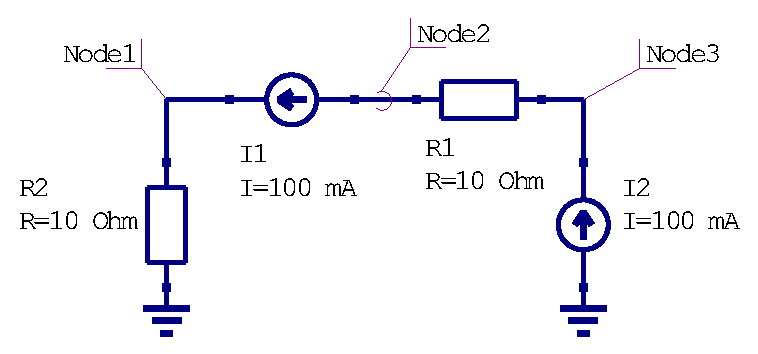
\includegraphics[width=10cm]{MNAsingular}
\end{center}
\caption{circuit with singular modified nodal analysis matrix}
\label{fig:MNAsingular}
\end{figure}
\FloatBarrier

The circuit in fig. \ref{fig:MNAsingular} has the following MNA
representation:
\begin{equation}
A x =
\begin{bmatrix}
\frac{1}{R_{2}} & 0 & 0\\
0 & \frac{1}{R_{1}} & -\frac{1}{R_{1}}\\
0 & -\frac{1}{R_{1}} & \frac{1}{R_{1}}
\end{bmatrix}
\cdot
\begin{bmatrix}
V_1\\
V_2\\
V_3
\end{bmatrix}
=
\begin{bmatrix}
0.1 & 0 & 0\\
0 & 0.1 & -0.1\\
0 & -0.1 & 0.1
\end{bmatrix}
\cdot
\begin{bmatrix}
V_1\\
V_2\\
V_3
\end{bmatrix}
=
\begin{bmatrix}
I_1\\
-I_1\\
I_2
\end{bmatrix}
=
\begin{bmatrix}
0.1\\
-0.1\\
0.1
\end{bmatrix}
=
z
\end{equation}

The second and third row of the matrix $A$ are linear dependent and
the matrix is singular because its determinant is zero.  Depending on
the right hand side $z$, the equation system has none or unlimited
solutions.  This is called an under-determined system.  The discussed
QR decomposition easily computes a valid solution without reducing
accuracy.  The LU decomposition would probably fail because of the
singularity.

\subsubsection{Least norm problem}
%\addcontentsline{toc}{subsubsection}{Least norm problem}

With some more effort it is possible to obtain the minimum-norm
solution of this problem.  The algorithm as described here would
probably yield the following solution:
\begin{equation}
x =
\begin{bmatrix}
V_1\\
V_2\\
V_3
\end{bmatrix}
=
\begin{bmatrix}
1\\
0\\
1
\end{bmatrix}
\end{equation}

This is one out of unlimited solutions.  The following short
description shows how it is possible to obtain the minimum-norm
solution.  When decomposing the transposed problem
\begin{equation}
A^T = Q\cdot R
\end{equation}

the minimum-norm solution $\hat{x}$ is obtained by forward substitution of
\begin{equation}
R^T\cdot x = z
\end{equation}

and multiplying the result with $Q$.
\begin{equation}
\hat{x} = Q\cdot x
\end{equation}

In the example above this algorithm results in a solution vector with
the least vector norm possible:
\begin{equation}
\hat{x} =
\begin{bmatrix}
V_1\\
V_2\\
V_3
\end{bmatrix}
=
\begin{bmatrix}
1\\
-0.5\\
0.5
\end{bmatrix}
\end{equation}

This algorithm outline is also sometimes called LQ decomposition
because of $R^T$ being a lower triangular matrix used by the forward
substitution.

\subsection{Jacobi method}
%\addcontentsline{toc}{subsection}{Jacobi method}

This method quite simply involves rearranging each equation to make
each variable a function of the other variables.  Then make an initial
guess for each solution and iterate.  For this method it is necessary
to ensure that all the diagonal matrix elements $a_{ii}$ are non-zero.
This is given for the nodal analysis and almostly given for the
modified nodal analysis.  If the linear equation system is solvable
this can always be achieved by rows substitutions.

\addvspace{12pt}

The algorithm for performing the iteration step $k + 1$ writes as
follows.
\begin{equation}
x_{i}^{(k+1)} = \dfrac{1}{a_{ii}}\left(z_i - \sum_{j=1}^{i-1} a_{ij}x_{j}^{(k)} - \sum_{j=i+1}^{n} a_{ij}x_{j}^{(k)}\right)
\;\;\;\; \textrm{ for } i = 1, \ldots, n
\end{equation}

This has to repeated until the new solution vectors $x^{(k+1)}$
deviation from the previous one $x^{(k)}$ is sufficiently small.

\addvspace{12pt}

The initial guess has no effect on whether the iterative method
converges or not, but with a good initial guess (as possibly given in
consecutive Newton-Raphson iterations) it converges faster (if it
converges).  To ensure convergence the condition
\begin{equation}
\sum_{j = 1, j \ne i}^{n} \left|a_{ij}\right| \le \left|a_{ii}\right|
\;\;\;\; \textrm{ for } i = 1, \ldots, n
\end{equation}

and at least one case
\begin{equation}
\sum_{i = 1, i \ne j}^{n} \left|a_{ij}\right| \le \left|a_{ii}\right|
\end{equation}

must apply.  If these conditions are not met, the iterative equations
may still converge.  If these conditions are met the iterative
equations will definitely converge.

\addvspace{12pt}

Another simple approach to a convergence criteria for iterative
algorithms is the Schmidt and v. Mises criteria.
\begin{equation}
\sqrt{\sum_{i = 1}^n \sum_{j = 1, j \ne i}^n \left|\dfrac{a_{ij}}{a_{ii}}\right|^2} < 1
\end{equation}

\subsection{Gauss-Seidel method}
%\addcontentsline{toc}{subsection}{Gauss-Seidel method}

The Gauss-Seidel algorithm is a modification of the Jacobi method.  It
uses the previously computed values in the solution vector of the same
iteration step.  That is why this iterative method is expected to
converge faster than the Jacobi method.

\addvspace{12pt}

The slightly modified algorithm for performing the $k + 1$ iteration
step writes as follows.
\begin{equation}
x_{i}^{(k+1)} = \dfrac{1}{a_{ii}}\left(z_i - \sum_{j=1}^{i-1} a_{ij}x_{j}^{(k+1)} - \sum_{j=i+1}^{n} a_{ij}x_{j}^{(k)}\right)
\;\;\;\; \textrm{ for } i = 1, \ldots, n
\end{equation}

The remarks about the initial guess $x^{(0)}$ as well as the
convergence criteria noted in the section about the Jacobi method
apply to the Gauss-Seidel algorithm as well.

\subsection{A comparison}
%\addcontentsline{toc}{subsection}{A comparison}

There are direct and iterative methods (algorithms) for solving linear
equation systems.  Equation systems with large and sparse matrices
should rather be solved with iterative methods.

\addvspace{12pt}

\begin{tabular}{|p{2.2cm}|p{1.5cm}|p{1.8cm}|p{2.1cm}|p{1.7cm}|p{2.95cm}|}
\hline
\raggedright method & \raggedleft precision & \raggedleft application & 
\raggedleft programming effort & \raggedleft computing complexity & 
\parbox[t]{2.95cm}{\raggedleft notes}\\
\hline
\raggedright Laplace expansion & \raggedleft numerical errors & 
\raggedleft general & \raggedleft straight forward &
\raggedleft $n!$ & \parbox[t]{2.95cm}{\raggedleft very time consuming}\\
\hline
\raggedright Gaussian elimination & \raggedleft numerical errors & 
\raggedleft general & \raggedleft intermediate & \raggedleft $n^3/3 + n^2/2$ &
\parbox[t]{2.95cm}{\raggedleft }\\
\hline
\raggedright Gauss-Jordan & \raggedleft numerical errors & \raggedleft general & \raggedleft intermediate & \raggedleft $n^3/3 + n^2 - n/3$ & \parbox[t]{2.95cm}{\raggedleft computes the inverse besides}\\
\hline
\raggedright LU decomposition & \raggedleft numerical errors & \raggedleft general & \raggedleft intermediate & \raggedleft $n^3/3 + n^2 - n/3$ & \parbox[t]{2.95cm}{\raggedleft useful for consecutive solutions}

\addvspace{1pt}

\\
\hline
\raggedright Jacobi & \raggedleft very good & \raggedleft diagonally dominant systems & \raggedleft easy & \raggedleft $n^2$ in each iteration step & \parbox[t]{2.95cm}{\raggedleft possibly no convergence}\\
\hline
\raggedright Gauss-Seidel & \raggedleft very good & \raggedleft diagonally dominant systems & \raggedleft easy & \raggedleft $n^2$ in each iteration step & \parbox[t]{2.95cm}{\raggedleft possibly no convergence}\\
\hline
\end{tabular}

\section{Extensions to the MNA}
%\addcontentsline{toc}{section}{Extensions to the MNA}
\label{sec:MNAext}

As noted in the previous sections the D matrix is zero and the B and C
matrices are transposed each other and filled with either 1, -1 or 0
provided that there are no dependent sources within the circuit.  This
changes when introducing active (and controlled) elements.

\subsection{Voltage controlled current source}
%\addcontentsline{toc}{subsection}{Voltage controlled current source}
\label{sec:vccs}

The voltage-dependent current source (VCCS), as shown in fig.
\ref{fig:vccs}, is determined by the following equation which
introduces one more unknown in the MNA matrix.

\begin{figure}[ht]
\begin{center}
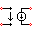
\includegraphics[width=4cm]{vccs}
\end{center}
\caption{voltage controlled current source}
\label{fig:vccs}
\end{figure}
\FloatBarrier

\begin{equation}
I_{out} = G\cdot\left(V_{1} - V_{2}\right)
\quad \rightarrow \quad
V_{1} - V_{4} - \frac{1}{G}\cdot I_{out} = 0
\label{eq:vccs}
\end{equation}

The new unknown variable $I_{out}$ must be considered by the four
remaining simple equations.

\begin{equation}
I_{1} = 0 \quad I_{2} = I_{out} \quad I_{3} = -I_{out} \quad I_{4} = 0
\end{equation}

And in matrix representation this is:
\begin{equation}
\label{eq:vccsStamp}
\begin{bmatrix}
.&.&.&.& 0\\
.&.&.&.& 1\\
.&.&.&.& -1\\
.&.&.&.& 0\\
1 & 0 & 0 & -1 & -\frac{1}{G}
\end{bmatrix}
\cdot
\begin{bmatrix}
V_{1}\\
V_{2}\\
V_{3}\\
V_{4}\\
I_{out}\\
\end{bmatrix}
=
\begin{bmatrix}
I_{1}\\
I_{2}\\
I_{3}\\
I_{4}\\
0\\
\end{bmatrix}
\end{equation}

As you can see the last row which has been added by the VCCS
represents the determining equation (\ref{eq:vccs}).  The additional
right hand column in the matrix keeps the system consistent.

\addvspace{12pt}

When pivotising the above MNA stamp \eqref{eq:vccsStamp} the
additional row and column can be saved ensuring $G$ keeps finite (the
pivot element must be non-zero).  Both representations are equivalent.
If $G$ is zero the below representation must be used.
\begin{equation}
\begin{bmatrix}
0&0&0&0\\
G&0&0&-G\\
-G&0&0&G\\
0&0&0&0
\end{bmatrix}
\cdot
\begin{bmatrix}
V_{1}\\
V_{2}\\
V_{3}\\
V_{4}\\
\end{bmatrix}
=
\begin{bmatrix}
I_{1}\\
I_{2}\\
I_{3}\\
I_{4}\\
\end{bmatrix}
\end{equation}

\subsection{Voltage controlled voltage source}
%\addcontentsline{toc}{subsection}{Voltage controlled voltage source}
\label{sec:vcvs}

The voltage-dependent voltage source (VCVS), as shown in fig.
\ref{fig:vcvs}, is determined by the following equation which
introduces one more unknown in the MNA matrix.

\begin{figure}[ht]
\begin{center}
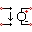
\includegraphics[width=4cm]{vcvs}
\end{center}
\caption{voltage controlled voltage source}
\label{fig:vcvs}
\end{figure}
\FloatBarrier

\begin{equation}
V_{2} - V_{3} = G\cdot \left(V_{1} - V_{4}\right)
\quad \rightarrow \quad
V_{1}\cdot G - V_{2} + V_{3} - V_{4}\cdot G = 0
\label{eq:vcvs}
\end{equation}

The new unknown variable $I_{out}$ must be considered by the four
remaining simple equations.

\begin{equation}
I_{1} = 0 \quad I_{2} = -I_{out} \quad I_{3} = I_{out} \quad I_{4} = 0
\end{equation}

And in matrix representation this is:
\begin{equation}
\begin{bmatrix}
.&.&.&.& 0\\
.&.&.&.& -1\\
.&.&.&.& 1\\
.&.&.&.& 0\\
G & -1 & 1 & -G & 0
\end{bmatrix}
\cdot
\begin{bmatrix}
V_{1}\\
V_{2}\\
V_{3}\\
V_{4}\\
I_{out}\\
\end{bmatrix}
=
\begin{bmatrix}
I_{1}\\
I_{2}\\
I_{3}\\
I_{4}\\
0\\
\end{bmatrix}
\end{equation}

\subsection{Current controlled current source}
%\addcontentsline{toc}{subsection}{Current controlled current source}
\label{sec:cccs}

The current-dependent current source (CCCS), as shown in fig.
\ref{fig:cccs}, is determined by the following equation which
introduces one more unknown in the MNA matrix.

\begin{figure}[ht]
\begin{center}
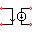
\includegraphics[width=4cm]{cccs}
\end{center}
\caption{current controlled current source}
\label{fig:cccs}
\end{figure}
\FloatBarrier

\begin{equation}
V_{1} - V_{4} = 0
\label{eq:cccs}
\end{equation}

The new unknown variable $I_{out}$ must be considered by the four
remaining simple equations.

\begin{equation}
I_{1} = +\frac{1}{G}\cdot I_{out} \quad I_{2} = I_{out} \quad I_{3} = -I_{out} \quad I_{4} = -\frac{1}{G}\cdot I_{out}
\end{equation}

And in matrix representation this is:
\begin{equation}
\begin{bmatrix}
.&.&.&.& \frac{1}{G}\\
.&.&.&.& 1\\
.&.&.&.& -1\\
.&.&.&.& -\frac{1}{G}\\
1 & 0 & 0 & -1 & 0
\end{bmatrix}
\cdot
\begin{bmatrix}
V_{1}\\
V_{2}\\
V_{3}\\
V_{4}\\
I_{out}\\
\end{bmatrix}
=
\begin{bmatrix}
I_{1}\\
I_{2}\\
I_{3}\\
I_{4}\\
0\\
\end{bmatrix}
\end{equation}

\subsection{Current controlled voltage source}
%\addcontentsline{toc}{subsection}{Current controlled voltage source}
\label{sec:ccvs}

The current-dependent voltage source (CCVS), as shown in fig.
\ref{fig:ccvs}, is determined by the following equations which
introduce two more unknowns in the MNA matrix.

\begin{figure}[ht]
\begin{center}
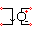
\includegraphics[width=4cm]{ccvs}
\end{center}
\caption{current controlled voltage source}
\label{fig:ccvs}
\end{figure}
\FloatBarrier

\begin{equation}
V_{1} - V_{4} = 0
\end{equation}
\begin{equation}
V_{2} - V_{3} = G\cdot I_{in}
\quad \rightarrow \quad
V_{2} - V_{3} - I_{in}\cdot G = 0
\label{eq:ccvs}
\end{equation}

The new unknown variables $I_{out}$ and $I_{in}$ must be considered by
the four remaining simple equations.

\begin{equation}
I_{1} = I_{in} \quad I_{2} = -I_{out} \quad I_{3} = I_{out} \quad I_{4} = -I_{in}
\end{equation}

The matrix representation needs to be augmented by two more new rows
(for the new unknown variables) and their corresponding columns.
\begin{equation}
\begin{bmatrix}
.&.&.&.& 1 & 0\\
.&.&.&.& 0 & -1\\
.&.&.&.& 0 & 1\\
.&.&.&.& -1 & 0\\
0 & 1 & -1 & 0 & -G & 0\\
1 & 0 & 0 & -1 & 0 & 0
\end{bmatrix}
\cdot
\begin{bmatrix}
V_{1}\\
V_{2}\\
V_{3}\\
V_{4}\\
I_{in}\\
I_{out}
\end{bmatrix}
=
\begin{bmatrix}
I_{1}\\
I_{2}\\
I_{3}\\
I_{4}\\
0\\
0
\end{bmatrix}
\end{equation}

\subsection{Operational amplifier}
%\addcontentsline{toc}{subsection}{Operational amplifier}

The ideal operational amplifier, as shown in fig. \ref{fig:opamp}, is
determined by the following equation which introduces one more unknown
in the MNA matrix.

\begin{figure}[ht]
\begin{center}
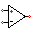
\includegraphics[width=4cm]{opamp}
\end{center}
\caption{ideal operational amplifier}
\label{fig:opamp}
\end{figure}
\FloatBarrier

\begin{equation}
V_{1} - V_{3} = 0
\label{eq:opamp}
\end{equation}

The new unknown variable $I_{out}$ must be considered by the three
remaining simple equations.

\begin{equation}
I_{1} = 0 \quad I_{2} = I_{out} \quad I_{3} = 0
\end{equation}

And in matrix representation this is:
\begin{equation}
\begin{bmatrix}
.&.&.& 0\\
.&.&.& 1\\
.&.&.& 0\\
1 & 0 & -1 & 0
\end{bmatrix}
\cdot
\begin{bmatrix}
V_{1}\\
V_{2}\\
V_{3}\\
I_{out}
\end{bmatrix}
=
\begin{bmatrix}
I_{1}\\
I_{2}\\
I_{3}\\
0
\end{bmatrix}
\end{equation}

The operational amplifier could be considered as a special case of a
voltage controlled current source with infinite forward
transconductance $G$.  Please note that the presented matrix form is
only valid in case where there is a finite feedback impedance
between the output and the inverting input port.

\addvspace{12pt}

To allow a feedback circuit to the non-inverting input (e.g.  for a
Schmitt trigger), one needs a limited output voltage swing.  The
following equations are often used to model the transmission
characteristic of operational amplifiers.
\begin{equation}
I_1 = 0 \qquad\qquad I_3 = 0
\end{equation}
\begin{equation}
\label{eq:OPVout}
V_2 = V_{max}\cdot\dfrac{2}{\pi}\arctan \left( \dfrac{\pi}{2\cdot V_{max}}\cdot G\cdot (V_1-V_3) \right)
\end{equation}

with $V_{max}$ being the maximum output voltage swing and $G$ the
voltage amplification.  To model the small-signal behaviour (AC
analysis), it is necessary to differentiate:
\begin{equation}
g = \dfrac{\partial V_2}{\partial (V_1-V_3)}
  = \dfrac{G}{1+\left( \dfrac{\pi}{2\cdot V_{max}}\cdot G\cdot (V_1-V_3) \right)^2}
\end{equation}

This leads to the following matrix representation being a specialised
three node voltage controlled voltage source (see section
\ref{sec:vcvs} on page \pageref{sec:vcvs}).
\begin{equation}
\begin{bmatrix}
.&.&.& 0\\
.&.&.& 1\\
.&.&.& 0\\
g & -1 & -g & 0
\end{bmatrix}
\cdot
\begin{bmatrix}
V_{1}\\
V_{2}\\
V_{3}\\
I_{out}
\end{bmatrix}
=
\begin{bmatrix}
I_{1}\\
I_{2}\\
I_{3}\\
0
\end{bmatrix}
\end{equation}

The above MNA matrix entries are also used during the non-linear DC
analysis with the 0 in the right hand side vector replaced by an
equivalent voltage
\begin{equation}
V_{eq} = g\cdot \left(V_1 - V_3\right) - V_{out}
\end{equation}
with $V_{out}$ computed using eq. \eqref{eq:OPVout}.

\addvspace{12pt}

With the given small-signal matrix representation, building the
S-parameters is easy.
\begin{equation}
(\underline{S}) =
\begin{bmatrix}
 1  &  0 & 0  \\
 4g & -1 & -4g\\
 0  &  0 &  1
\end{bmatrix}
\end{equation}

\subsection{Transformer}
%\addcontentsline{toc}{subsection}{Transformer}

The two winding ideal transformer, as shown in fig.
\ref{fig:actrafo}, is determined by the following equation which
introduces one more unknown in the MNA matrix.

\begin{figure}[ht]
\begin{center}
\includegraphics[width=4cm]{actrafo}
\end{center}
\caption{ideal two winding transformer}
\label{fig:actrafo}
\end{figure}
\FloatBarrier

\begin{equation}
T\cdot\left(V_{2} - V_{3}\right) = V_{1} -V_{4}
\quad \rightarrow \quad
V_{1} - T\cdot V_{2} + T\cdot V_{3} - V_{4} = 0
\label{eq:trafo}
\end{equation}

The new unknown variable $I_{t}$ must be considered by the four
remaining simple equations.

\begin{equation}
I_{1} = -I_{t} \quad I_{2} = T\cdot I_{t} \quad I_{3} = -T\cdot I_{t} \quad I_{4} = I_{t}
\end{equation}

And in matrix representation this is:
\begin{equation}
\begin{bmatrix}
.&.&.&.& -1\\
.&.&.&.& T\\
.&.&.&.& -T\\
.&.&.&.& 1\\
1 & -T & T & -1 & 0
\end{bmatrix}
\cdot
\begin{bmatrix}
V_{1}\\
V_{2}\\
V_{3}\\
V_{4}\\
I_{t}
\end{bmatrix}
=
\begin{bmatrix}
I_{1}\\
I_{2}\\
I_{3}\\
I_{4}\\
0
\end{bmatrix}
\end{equation}

It is noticeable that the additional row (part of the C matrix) and the
corresponding column (part of the B matrix) are transposed to each
other.  When considering the turns ratio $T$ being complex introducing
an additional phase the transformer can be used as phase-shifting
transformer.  Both the vectors must be conjugated complex transposed
in this case.

\subsection{Symmetrical transformer}
%\addcontentsline{toc}{subsection}{Symmetrical transformer}

The ideal symmetrical transformer, as shown in fig.
\ref{fig:acstrafo}, is determined by the following equations which
introduce two more unknowns in the MNA matrix.

\begin{figure}[ht]
\begin{center}
\includegraphics[width=4cm]{acstrafo}
\end{center}
\caption{ideal three winding transformer}
\label{fig:acstrafo}
\end{figure}
\FloatBarrier

\begin{equation}
T_{1}\cdot\left(V_{2} - V_{3}\right) = V_{1} - V_{6}
\quad \rightarrow \quad
V_{1} - T_{1}\cdot V_{2} + T_{1}\cdot V_{3} - V_{6} = 0
\end{equation}
\begin{equation}
T_{2}\cdot\left(V_{2} - V_{3}\right) = V_{5} - V_{4}
\quad \rightarrow \quad
- T_{2}\cdot V_{2} + T_{2}\cdot V_{3} - V_{4} + V_{5} = 0
\label{eq:acstrafo}
\end{equation}

The new unknown variables $I_{T1}$ and $I_{T2}$ must be considered by
the six remaining simple equations.
\begin{equation}
I_{2} = T_{1}\cdot I_{T1} + T_{2}\cdot I_{T2} \quad I_{3} = -T_{1}\cdot I_{T1} - T_{2}\cdot I_{T2}
\end{equation}
\begin{equation}
I_{1} = -I_{T1} \quad I_{4} = I_{T2} \quad I_{5} = -I_{T2} \quad I_{6} = I_{T1}
\end{equation}

The matrix representation needs to be augmented by two more new rows
and their corresponding columns.
\begin{equation}
\begin{bmatrix}
.&.&.&.&.&.& -1 & 0\\
.&.&.&.&.&.& T_{1} & T_{2}\\
.&.&.&.&.&.& -T_{1} & -T_{2}\\
.&.&.&.&.&.& 0 & 1\\
.&.&.&.&.&.& 0 & -1\\
.&.&.&.&.&.& 1 & 0\\
1 & -T_{1} & T_{1} & 0 & 0 & -1 & 0 & 0\\
0 & -T_{2} & T_{2} & -1 & 1 & 0 & 0 & 0
\end{bmatrix}
\cdot
\begin{bmatrix}
V_{1}\\
V_{2}\\
V_{3}\\
V_{4}\\
V_{5}\\
V_{6}\\
I_{T1}\\
I_{T2}
\end{bmatrix}
=
\begin{bmatrix}
I_{1}\\
I_{2}\\
I_{3}\\
I_{4}\\
I_{5}\\
I_{6}\\
0\\
0
\end{bmatrix}
\end{equation}

\subsection{Gyrator}
%\addcontentsline{toc}{subsection}{Gyrator}

The ideal gyrator, as shown in fig. \ref{fig:gyrator}, is determined
by the following equations which introduce two more unknowns in the
MNA matrix.

\begin{figure}[ht]
\begin{center}
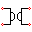
\includegraphics[width=4cm]{gyrator}
\end{center}
\caption{ideal gyrator}
\label{fig:gyrator}
\end{figure}
\FloatBarrier

\begin{equation}
I_{in} = \frac{1}{R}\cdot\left(V_{2} - V_{3}\right)
\quad \rightarrow \quad
\frac{1}{R}\cdot V_{2} - \frac{1}{R}\cdot V_{3} - I_{in} = 0
\end{equation}
\begin{equation}
I_{out} = -\frac{1}{R}\cdot\left(V_{1} - V_{4}\right)
\quad \rightarrow \quad
-\frac{1}{R}\cdot V_{1} + \frac{1}{R}\cdot V_{4} - I_{out} = 0
\label{eq:gyrator}
\end{equation}

The new unknown variables $I_{out}$ and $I_{in}$ must be considered by
the four remaining simple equations.

\begin{equation}
I_{1} = I_{in} \quad I_{2} = I_{out} \quad I_{3} = -I_{out} \quad I_{4} = -I_{in}
\end{equation}

The matrix representation needs to be augmented by two more new rows
(for the new unknown variables) and their corresponding columns.
\begin{equation}
\label{eq:gyratorStamp}
\begin{bmatrix}
.&.&.&.& 1 & 0\\
.&.&.&.& 0 & 1\\
.&.&.&.& 0 & -1\\
.&.&.&.& -1 & 0\\
0 & \frac{1}{R} & -\frac{1}{R} & 0 & -1 & 0\\
-\frac{1}{R} & 0 & 0 & \frac{1}{R} & 0 & -1
\end{bmatrix}
\cdot
\begin{bmatrix}
V_{1}\\
V_{2}\\
V_{3}\\
V_{4}\\
I_{in}\\
I_{out}
\end{bmatrix}
=
\begin{bmatrix}
I_{1}\\
I_{2}\\
I_{3}\\
I_{4}\\
0\\
0
\end{bmatrix}
\end{equation}

The above gyrators MNA stamp \eqref{eq:gyratorStamp} can be pivotised
with no further conditions and yields the following representation
saving both augmentations.
\begin{equation}
\begin{bmatrix}
0&\frac{1}{R}&-\frac{1}{R}&0\\
-\frac{1}{R}&0&0&\frac{1}{R}\\
\frac{1}{R}&0&0&-\frac{1}{R}\\
0&-\frac{1}{R}&\frac{1}{R}&0
\end{bmatrix}
\cdot
\begin{bmatrix}
V_{1}\\
V_{2}\\
V_{3}\\
V_{4}
\end{bmatrix}
=
\begin{bmatrix}
I_{1}\\
I_{2}\\
I_{3}\\
I_{4}
\end{bmatrix}
\end{equation}

\subsection{Attenuator}
%\addcontentsline{toc}{subsection}{Attenuator}

The ideal attenuator with (power) attenuation $L$ is determined by the
following Z parameters.

\begin{equation}
Z_{11} = Z_{22} = Z_{ref}\cdot\frac{L+1}{L-1}
\end{equation}
\begin{equation}
Z_{12} = Z_{21} = Z_{ref}\cdot\frac{2\cdot\sqrt{L}}{L-1}
\end{equation}

The MNA matrix representation can be derived from the Z parameters in the
following way.
\begin{equation}
\begin{bmatrix}
 . & .  &  1 & 0\\
 . & .  &  0 & 1\\
-1 &  0 & Z_{11} & Z_{12}\\
 0 & -1 & Z_{21} & Z_{22}
\end{bmatrix}
\cdot
\begin{bmatrix}
V_{1}\\
V_{2}\\
I_{in}\\
I_{out}
\end{bmatrix}
=
\begin{bmatrix}
I_{1}\\
I_{2}\\
0\\
0
\end{bmatrix}
\end{equation}


The Z parameter representation is not very practical as new lines
in the MNA matrix have to be added. More useful are the Y parameters.

\begin{equation}
\frac{1}{Z_{ref}\cdot (L-1)}\cdot
\begin{bmatrix}
 L+1            & -2\cdot\sqrt{L} \\
-2\cdot\sqrt{L} & L+1
\end{bmatrix}
\cdot
\begin{bmatrix}
V_{1}\\
V_{2}
\end{bmatrix}
=
\begin{bmatrix}
I_{1}\\
I_{2}
\end{bmatrix}
\end{equation}



\subsection{Isolator}
%\addcontentsline{toc}{subsection}{Isolator}

The ideal isolator with reference impedances $Z_1$ (input) and $Z_2$
(output) is determined by the following Z parameters.

\begin{equation}
Z_{11} = Z_1  \qquad
Z_{12} = 0
\end{equation}
\begin{equation}
Z_{21} = 2\cdot\sqrt{Z_1\cdot Z_2}  \qquad
Z_{22} = Z_2
\end{equation}

The MNA matrix representation can be derived from the Z parameters in the
following way.
\begin{equation}
\begin{bmatrix}
 . & .  & 1  & 0 \\
 . & .  &  0 & 1 \\
-1 &  0 & Z_{11} & Z_{12}\\
 0 & -1 & Z_{21} & Z_{22}
\end{bmatrix}
\cdot
\begin{bmatrix}
V_{1}\\
V_{2}\\
I_{in}\\
I_{out}
\end{bmatrix}
=
\begin{bmatrix}
I_{1}\\
I_{2}\\
0\\
0
\end{bmatrix}
\end{equation}

A more useful MNA representation is with Y parameters.

\begin{equation}
\begin{bmatrix}
 1/Z_1 & 0 \\
 -2/\sqrt{Z_1\cdot Z_2} & 1/Z_2
\end{bmatrix}
\cdot
\begin{bmatrix}
V_{1}\\
V_{2}
\end{bmatrix}
=
\begin{bmatrix}
I_{1}\\
I_{2}
\end{bmatrix}
\end{equation}



\subsection{Amplifier}
%\addcontentsline{toc}{subsection}{Amplifier}

The ideal amplifier is an isolator with voltage gain $G$ and is
determined by the following Z or Y parameters.

\begin{equation}
Z_{11} = Z_1  \qquad
Z_{12} = 0
\end{equation}
\begin{equation}
Z_{21} = 2\cdot\sqrt{Z_1\cdot Z_2}\cdot G  \qquad
Z_{22} = Z_2
\end{equation}
\begin{equation}
Y_{11} = \frac{1}{Z_1}  \qquad
Y_{12} = 0
\end{equation}
\begin{equation}
Y_{21} = -\frac{2\cdot G}{\sqrt{Z_1\cdot Z_2}}  \qquad
Y_{22} = \frac{1}{Z_2}
\end{equation}

\subsection{Phase Shifter}
%\addcontentsline{toc}{subsection}{Phase Shifter}

A phase shifter alters the phase of the input signal independently on
the frequency.  As a result the relation between input and output
signal is complex.  To get the DC model, some simulators use the AC
formulas and create the real part or the magnitude.  This procedure
has no physical reason, because it uses an operation that is not
defined for DC.  But one can think in the following direction: As a DC
quantity is constant, it doesn't change if it is phase-shifted.  (An
AC quantity doesn't change it magnitude, too.)  Or to say it with
other words, for a DC simulation the phase to shift is always zero.
That leads to the result that the phase shifter is a short circuit for
DC.  So, this is true for all reference impedances.

\subsection{Circulator}
%\addcontentsline{toc}{subsection}{Circulator}

The ideal circulator cannot be characterized with Z or Y parameters,
because their values are partly infinite.  But implementing with S
parameters is practical (see chapter \ref{sec:CirculatorSparameter}
for S parameters of the circulator).
\begin{equation}
\begin{bmatrix}
 . & . & .  &  1 & 0 & 0\\
 . & . & .  &  0 & 1 & 0\\
 . & . & .  &  0 & 0 & 1\\
S_{11}-1 &  S_{12} & S_{13} & Z_0\cdot (S_{11}+1) & Z_0\cdot S_{12} & Z_0\cdot S_{13}\\
S_{21} &  S_{22}-1 & S_{23} & Z_0\cdot S_{21} & Z_0\cdot (S_{22}+1) & Z_0\cdot S_{23}\\
S_{31} &  S_{32} & S_{33}-1 & Z_0\cdot S_{31} & Z_0\cdot S_{32} & Z_0\cdot (S_{33}+1)
\end{bmatrix}
\cdot
\begin{bmatrix}
V_{1}\\
V_{2}\\
V_{3}\\
I_{I1}\\
I_{I2}\\
I_{I3}
\end{bmatrix}
=
\begin{bmatrix}
I_{1}\\
I_{2}\\
I_{3}\\
0\\
0\\
0
\end{bmatrix}
\end{equation}

\subsection{Bias T}
%\addcontentsline{toc}{subsection}{Bias T}

The MNA matrix of an ideal bias t (with ports as shown in
fig. \ref{fig:biast}) writes as follows:
\begin{equation}
\begin{bmatrix}
 . & . & .  &  0\\
 . & . & .  &  1\\
 . & . & .  & -1\\
 0 & 1 & -1 &  0
\end{bmatrix}
\cdot
\begin{bmatrix}
V_{1}\\
V_{2}\\
V_{3}\\
I_{out}
\end{bmatrix}
=
\begin{bmatrix}
I_{1}\\
I_{2}\\
I_{3}\\
0
\end{bmatrix}
\end{equation}

\section{Non-linear DC Analysis}
%\addcontentsline{toc}{section}{Non-linear DC Analysis}

Previous sections described using the modified nodal analysis solving
linear networks including controlled sources.  It can also be used to
solve networks with non-linear components like diodes and transistors.
Most methods are based on iterative solutions of a linearised equation
system.  The best known is the so called Newton-Raphson method.

\subsection{Newton-Raphson method}
%\addcontentsline{toc}{subsection}{Newton-Raphson method}
\label{sec:NRmethod}

The Newton-Raphson method is going to be introduced using the example
circuit shown in fig. \ref{fig:NLexample} having a single unknown: the
voltage at node 1.

\begin{figure}[ht]
\begin{center}
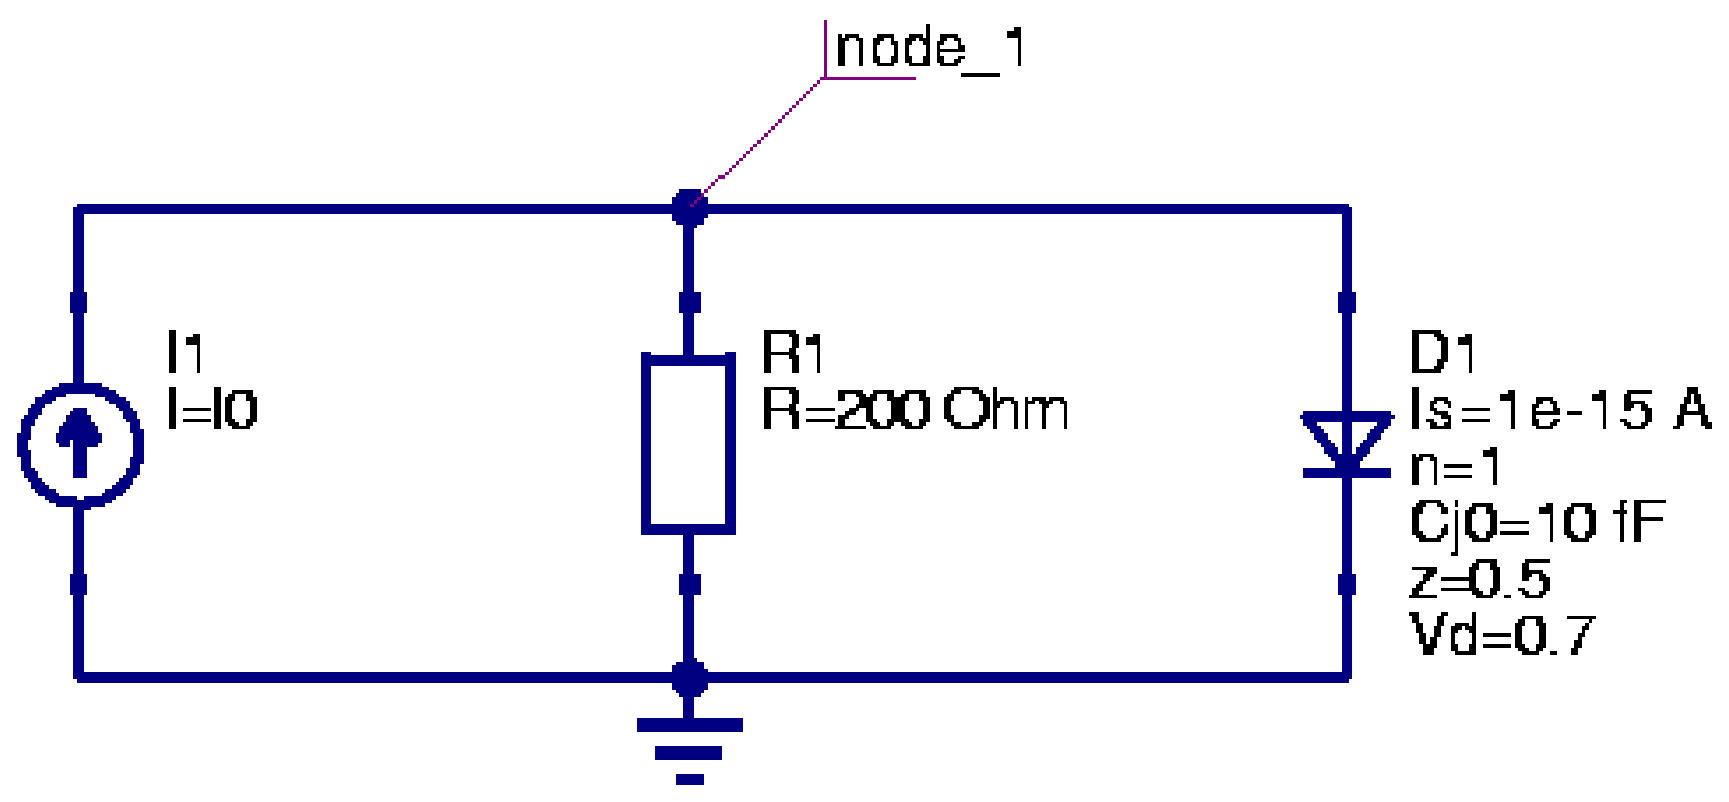
\includegraphics[width=10cm]{NLexample}
\end{center}
\caption{example circuit for non-linear DC analysis}
\label{fig:NLexample}
\end{figure}
\FloatBarrier

The 1x1 MNA equation system to be solved can be written as
\begin{equation}
\begin{bmatrix}
G
\end{bmatrix}
\cdot
\begin{bmatrix}
V_{1}
\end{bmatrix}
=
\begin{bmatrix}
I_{0}
\end{bmatrix}
\label{eq:NLmatrix}
\end{equation}

whereas the value for $G$ is now going to be explained.  The current
through a diode is simply determined by Schockley's approximation
\begin{equation}
I_{d} = I_{S}\cdot \left(e^{\frac{V_{d}}{V_{T}}} - 1\right)
\end{equation}

Thus Kirchhoff's current law at node 1 can be expressed as
\begin{equation}
I_{0} = \dfrac{V}{R} + I_{S}\cdot \left(e^{\frac{V}{V_{T}}} - 1\right)
\end{equation}

By establishing eq. (\ref{eq:NLfunc}) it is possible to trace the
problem back to finding the zero point of the function $f$.
\begin{equation}
f(V) = \dfrac{V}{R} + I_{S}\cdot \left(e^{\frac{V}{V_{T}}} - 1\right) - I_{0}
\label{eq:NLfunc}
\end{equation}

Newton developed a method stating that the zero point of a functions
derivative (i.e. the tangent) at a given point is nearer to the zero
point of the function itself than the original point.  In mathematical
terms this means to linearise the function $f$ at a starting value
$V^{(0)}$.
\begin{equation}
f\left(V^{(0)} + \Delta V\right) \approx f\left(V^{(0)}\right) + \left.\dfrac{\partial f\left(V\right)}{\partial V}\right|_{V^{(0)}}\cdot \Delta V
\;\;\;\; \text{ with } \;\;\;\;
\Delta V = V^{(1)} - V^{(0)}
\label{eq:NRapprox}
\end{equation}

Setting $f(V^{(1)}) = 0$ gives
\begin{equation}
V^{(1)} = V^{(0)} - \dfrac{f\left(V^{(0)}\right)}{\left.\dfrac{\partial f\left(V\right)}{\partial V}\right|_{V^{(0)}}}
\end{equation}

or in the general case with $m$ being the number of iteration
\begin{equation}
V^{(m + 1)} = V^{(m)} - \dfrac{f\left(V^{(m)}\right)}{\left.\dfrac{\partial f\left(V\right)}{\partial V}\right|_{V^{(m)}}}
\label{eq:NRgeneral}
\end{equation}

This must be computed until $V^{(m+1)}$ and $V^{(m)}$ differ less than a
certain barrier.
\begin{equation}
\left|V^{(m+1)} - V^{(m)}\right| < \varepsilon_{abs} + \varepsilon_{rel}\cdot \left|V^{(m)}\right|
\label{eq:NLconvergence}
\end{equation}

With very small $\varepsilon_{abs}$ the iteration would break too
early and for little $\varepsilon_{rel}$ values the iteration aims to
a useless precision for large absolute values of $V$.

\begin{figure}[ht]
\begin{center}
\psfrag{V0}{$\mathrm{V^{(0)}}$}
\psfrag{V1}{$\mathrm{V^{(1)}}$}
\psfrag{V2}{$\mathrm{V^{(2)}}$}
\includegraphics[width=0.75\linewidth]{newton}
\end{center}
\caption{Newton-Raphson method for example circuit}
\label{fig:NewtonRaphson}
\end{figure}
\FloatBarrier

With this theoretical background it is now possible to step back to
eq. (\ref{eq:NLfunc}) being the determining equation for the example
circuit.  With
\begin{equation}
g_{d}^{(m)} = \left.\dfrac{\partial I_{d}}{\partial V}\right|_{V^{(m)}} = \dfrac{I_{S}}{V_{T}}\cdot e^{\frac{V^{(m)}}{V_{T}}}
\end{equation}

and
\begin{equation}
\left.\dfrac{\partial f\left(V\right)}{\partial V}\right|_{V^{(m)}} = \dfrac{1}{R} + g_{d}^{(m)}
\end{equation}

the eq. (\ref{eq:NRgeneral}) can be written as
\begin{equation}
\left(g_{d}^{(m)} + \dfrac{1}{R}\right)\cdot V^{(m+1)} = I_{0} - \left(I_{d}^{(m)} - g_{d}^{(m)}\cdot V^{(m)}\right)
\label{eq:NRresult}
\end{equation}

when the expression
\begin{equation}
f\left(V^{(m)}\right) = \dfrac{1}{R}\cdot V^{(m)} + I_{d}^{(m)} - I_{0}
\end{equation}

based upon eq. (\ref{eq:NLfunc}) is taken into account.  Comparing the
introductory MNA equation system in eq. (\ref{eq:NLmatrix}) with
eq. (\ref{eq:NRresult}) proposes the following equivalent circuit for
the diode model.

\begin{figure}[ht]
\begin{center}
\psfrag{gd}{$\mathrm{g_{d}^{(m)}}$}
\psfrag{Ieq}{$\mathrm{I_{d}^{(m)} - g_{d}^{(m)}\cdot V^{(m)}}$}
\includegraphics[width=0.2\linewidth]{newtondiode}
\end{center}
\caption{accompanied equivalent circuit for intrinsic diode}
\label{fig:AccompaniedModel}
\end{figure}
\FloatBarrier

\label{sec:DCdiode}

With
\begin{equation}
I_{eq} = I_{d}^{(m)} - g_{d}^{(m)}\cdot V^{(m)}
\end{equation}

the MNA matrix entries can finally be written as
\begin{equation}
\begin{bmatrix}
g_{d} & -g_{d}\\
-g_{d} & g_{d}
\end{bmatrix}
\cdot
\begin{bmatrix}
V_{1}\\
V_{2}
\end{bmatrix}
=
\begin{bmatrix}
-I_{eq}\\
I_{eq}
\end{bmatrix}
\end{equation}

In analog ways all controlled current sources with non-linear
current-voltage dependency built into diodes and transistors can be
modeled.  The left hand side of the MNA matrix (the A matrix) is
called Jacobian matrix which is going to be build in each iteration
step.  For the solution vector $x$ possibly containing currents as
well when voltage sources are in place a likely convergence criteria
as defined in eq. (\ref{eq:NLconvergence}) must be defined for the
currents.

\addvspace{12pt}

Having understood the one-dimensional example, it is now only a
small step to the general multi-dimensional algorithm: The node
voltage becomes a vector $\boldsymbol{V}^{(m)}$, factors become
the corresponding matrices and differentiations become Jacobian
matrices.

\addvspace{12pt}

The function whose zero must be found is the transformed MNA
equation \ref{eq:NLmatrix}:

\begin{equation}
\boldsymbol{f}( \boldsymbol{V}^{(m)} ) =
    \boldsymbol{G}\cdot \boldsymbol{V}^{(m)} - \boldsymbol{I}_{0}
\end{equation}

In addition to the linear case, the vector $\boldsymbol{I}_{0}$
contains the currents flowing into the non-linear components.
The iteration formula of the Newton-Raphson method writes:

\begin{equation}
\boldsymbol{V}^{(m+1)} = \boldsymbol{V}^{(m)} -
  \left( \left.\frac{\partial\boldsymbol{f}( \boldsymbol{V} )}
                    {\partial\boldsymbol{V}}\right|_{V^{(m)}} \right)^{-1}
  \cdot \boldsymbol{f}( \boldsymbol{V}^{(m)} )
\label{eq:ndimNewton}
\end{equation}

Note that the Jacobian matrix is nothing else but the real
part of the MNA matrix for the AC analysis:

\begin{equation}
\boldsymbol{J}^{(m)}
  = \left.\frac{\partial\boldsymbol{f}( \boldsymbol{V} )}
               {\partial\boldsymbol{V}}\right|_{\boldsymbol{V}^{(m)}}
  = \text{Re}\left(\boldsymbol{G}_{AC}\right)
\end{equation}

The disadvantage of the formula \ref{eq:ndimNewton} is the fact
that for each iteration the matrix $\boldsymbol{f}( \boldsymbol{V}^{(m)} )$
has to be built even with the constant values of the linear
components. This can be avoided. Multiplying equation
\ref{eq:ndimNewton} with the Jacobian leads to

\begin{equation}
\boldsymbol{J}^{(m)} \cdot \boldsymbol{V}^{(m+1)}
  = \boldsymbol{J}^{(m)} \cdot \boldsymbol{V}^{(m)} -
    \boldsymbol{f}( \boldsymbol{V}^{(m)} )
\end{equation}

As can be seen, the linear terms on the right side cancel
each other. So, bringing the Jacobian back to the right side
results in the new iteration formula:
\begin{equation}
\boldsymbol{V}^{(m+1)} = \left( \boldsymbol{J}^{(m)} \right)^{-1} -
  \left( \boldsymbol{J}_{nl}^{(m)}\cdot \boldsymbol{V}^{(m)} - \boldsymbol{I}_{nl}^{(m)} \right)
\end{equation}

where the index $nl$ denotes only the non-linear terms.


\subsection{Convergence}
%\addcontentsline{toc}{subsection}{Convergence}
\label{sec:convergenceDC}

Numerical as well as convergence problems occur during the
Newton-Raphson iterations when dealing with non-linear device curves
as they are used to model the DC behaviour of diodes and transistors.

\addvspace{12pt}

Linearising the exponential diode eq. \eqref{eq:curve} in the forward
region a numerical overflow can occur.  The diagram in
fig. \ref{fig:NewtonBad} visualises this situation.  Starting with
$V^{(0)}$ the next iteration value gets $V^{(1)}$ which results in an
indefinite large diode current.  It can be limited by iterating in
current instead of voltage when the computed voltage exceeds a certain
value.

\addvspace{12pt}

How this works is going to be explained using the diode model shown in
fig. \ref{fig:AccompaniedModel}.  When iterating in voltage (as
normally done) the new diode current is

\begin{equation}
\hat{I}_{d}^{(m+1)} = g_{d}^{(m)} \left(\hat{V}^{(m+1)} - V^{(m)}\right) + I_{d}^{(m)}
\end{equation}

The computed value $\hat{V}^{(m+1)}$ in iteration step $m+1$ is not
going to be used for the following step when $V^{(m)}$ exceeds the
critical voltage $V_{CRIT}$ which gets explained in the below
paragraphs.  Instead, the value resulting from

\begin{equation}
I_{d}^{(m+1)} = I_{S}\cdot \left(e^{\frac{V^{(m+1)}}{n V_{T}}} - 1\right)
\end{equation}

is used (i.e. iterating in current).  With

\begin{equation}
\hat{I}_{d}^{(m+1)} \; \shortstack{!\\=} \; I_{d}^{(m+1)}
\;\;\;\; \text{ and } \;\;\;\;
g_{d}^{(m)} = \dfrac{I_{S}}{n\cdot V_{T}}\cdot e^{\frac{V^{(m)}}{n\cdot V_{T}}}
\end{equation}

the new voltage can be written as

\begin{equation}
V^{(m+1)} = V^{(m)} + n V_{T}\cdot \ln{\left(\dfrac{\hat{V}^{(m+1)} - V^{(m)}}{n V_{T}} + 1\right)}
\end{equation}

Proceeding from Shockley's simplified diode equation the critical
voltage is going to be defined.  The explained algorithm can be used
for all exponential DC equations used in diodes and transistors.

\begin{align}
I\left(V\right) &= I_{S}\cdot \left(e^{\frac{V}{n V_{T}}} - 1\right)
\label{eq:curve}\\
y\left(x\right) &= f \left(x\right)
\label{eq:explicit}
\end{align}

\begin{figure}[ht]
\begin{center}
\psfrag{V0}{$\mathrm{V^{(0)}}$}
\psfrag{V1}{$\mathrm{V^{(1)}}$}
\psfrag{V2}{$\mathrm{V^{(2)}}$}
\psfrag{VCRIT}{$\mathrm{V_{CRIT} \rightarrow}$}
\includegraphics[width=0.75\linewidth]{newtonbad}
\end{center}
\caption{numerical problem with Newton-Raphson algorithm}
\label{fig:NewtonBad}
\end{figure}
\FloatBarrier

The critical voltage $V_{CRIT}$ is the voltage where the curve radius
of eq. \eqref{eq:curve} has its minimum with $I$ and $V$ having
equally units.  The curve radius $R$ for the explicit definition in
eq. \eqref{eq:explicit} can be written as

\begin{equation}
R = \left|\dfrac{\left(1+\left(\dfrac{dy}{dx}\right)^{2}\right)^{3/2}}{\dfrac{d^{2}y}{dx^{2}}}\right|
\label{eq:radius}
\end{equation}

Finding this equations minimum requires the derivative.

\begin{equation}
\dfrac{dR}{dx} = \dfrac{\dfrac{d^{2}y}{dx^{2}} \cdot \dfrac{3}{2}\left(1+\left(\dfrac{dy}{dx}\right)^{2}\right)^{1/2} \cdot 2 \cdot \dfrac{dy}{dx} \cdot \dfrac{d^{2}y}{dx^{2}} - \left(1+\left(\dfrac{dy}{dx}\right)^{2}\right)^{3/2} \cdot \dfrac{d^{3}y}{dx^{3}}}{\left(\dfrac{d^{2}y}{dx^{2}}\right)^{2}}
\label{eq:radiusderivative}
\end{equation}

The diagram in fig. \ref{fig:radius} shows the graphs of
eq. \eqref{eq:radius} and eq. \eqref{eq:radiusderivative} with $n=1$,
$I_{S}=100\nano\ampere$ and $V_{T}=25\milli\volt$.

\begin{figure}[ht]
\begin{center}
\includegraphics[width=0.7\linewidth]{radius}
\end{center}
\caption{curve radius of exponential diode curve and its derivative}
\label{fig:radius}
\end{figure}
\FloatBarrier

With the following higher derivatives of eq. \eqref{eq:curve}

\begin{align}
\dfrac{d I\left(V\right)}{dV} &= \dfrac{I_{S}}{n V_{T}}\cdot e^{\frac{V}{n V_{T}}}\\
\dfrac{d^{2} I\left(V\right)}{dV^{2}} &= \dfrac{I_{S}}{n^{2} V_{T}^{2}}\cdot e^{\frac{V}{n V_{T}}}\\
\dfrac{d^{3} I\left(V\right)}{dV^{3}} &= \dfrac{I_{S}}{n^{3} V_{T}^{3}}\cdot e^{\frac{V}{n V_{T}}}
\end{align}

the critical voltage results in

\begin{equation}
\dfrac{dR}{dx} \;\shortstack{!\\=}\; 0 = 3 - \dfrac{n^{2} V_{T}^{2}}{I_{S}^{2}}\cdot e^{-2\frac{V}{n V_{T}}} - 1
\;\;\;\; \rightarrow \;\;\;\;
V_{CRIT} = n V_{T}\cdot \ln{\left(\dfrac{n V_{T}}{I_{S} \sqrt{2}}\right)}
\end{equation}

In order to avoid numerical errors a minimum value of the
pn-junction's derivative (i.e. the currents tangent in the operating
point) $g_{min}$ is defined.  On the one hand this avoids very large
deviations of the appropriate voltage in the next iteration step in
the backward region of the pn-junction and on the other hand it avoids
indefinite large voltages if $g_d$ itself suffers from numerical
errors and approaches zero.

\addvspace{12pt}

The quadratic input I-V curve of field-effect transistors as well as
the output characteristics of these devices can be handled in similar
ways.  The limiting (and thereby improving the convergence behaviour)
algorithm must somehow ensure that the current and/or voltage
deviation from one iteration step to the next step is not too a large
value.  Because of the wide range of existing variations how these
curves are exactly modeled there is no standard strategy to achieve
this.  Anyway, the threshold voltage $V_{Th}$ should play an important
role as well as the direction which the current iteration step
follows.
